\chapter[Project Implementation]{PROJECT IMPLEMENTATION}

\section{Environment Setup}

For the implementation of our proposed model, AIRVTON, we meticulously crafted a robust computing environment tailored to meet the demanding requirements of training deep neural networks. The following comprehensive details outline the setup utilized during the implementation phase:

\subsection{Hardware Configuration}
\begin{itemize}
  \item \textbf{CPU}: Intel Core i7-10700K, featuring 8 cores and 16 threads, clocked at 3.80 GHz, providing ample computational power for parallel processing tasks.
  \item \textbf{GPU}: NVIDIA GeForce RTX 3090, equipped with 24GB of ultra-fast GDDR6X VRAM, harnessing the immense parallel computing capabilities of CUDA cores for accelerated deep learning computations.
  \item \textbf{RAM}: 64GB of high-speed DDR4 memory operating at 3200 MHz, ensuring sufficient memory capacity to accommodate large datasets and deep neural network models.
  \item \textbf{Storage}: A blazing-fast 1TB NVMe SSD facilitated swift data access and storage operations, minimizing latency and bottlenecks during training and inference phases.
\end{itemize}

\subsection{Software Stack}
\begin{itemize}
  \item \textbf{Operating System}: Ubuntu 20.04 LTS (64-bit), renowned for its stability, security, and compatibility with deep learning frameworks.
  \item \textbf{Deep Learning Framework}: PyTorch 1.9.0, coupled with CUDA support, provided a flexible and efficient platform for developing and training neural network models, leveraging GPU acceleration for enhanced performance.
  \item \textbf{Additional Libraries}: NumPy, SciPy, and Matplotlib were instrumental for data manipulation, scientific computing, and visualization tasks, enhancing the functionality of PyTorch.
  \item \textbf{Image Processing Tools}: OpenCV, a versatile library for computer vision tasks, facilitated image loading, preprocessing, crucial for preparing datasets for training and evaluation.
  \item \textbf{Environment Management}: Anaconda virtual environment served as a robust solution for package management and isolation, enabling seamless configuration and reproducibility across different computing environments.
\end{itemize}

\subsection{Dependency Installation}
\begin{itemize}
  \item PyTorch and CUDA Toolkit were installed via Anaconda using the following commands, ensuring compatibility and optimized performance with the NVIDIA GPU:
    \begin{verbatim}
    conda install cudatoolkit=11.1 -c nvidia
    \end{verbatim}
    \begin{verbatim}
    conda install pytorch torchvision torchaudio -c pytorch
    \end{verbatim}


  \item Additional Python dependencies, including NumPy, SciPy, Matplotlib, and OpenCV, were installed using the \texttt{pip} package manager to complement the deep learning framework:
    \begin{verbatim}
    pip install numpy scipy matplotlib opencv-python
    \end{verbatim}
\end{itemize}

This meticulously configured environment served as the cornerstone for executing our ambitious project, enabling the seamless integration of cutting-edge deep learning techniques for fashion recommendation and virtual try-on tasks. Leveraging the computational prowess of the NVIDIA GeForce RTX 3090 GPU and the optimized performance of PyTorch with CUDA support, we embarked on a journey to push the boundaries of innovation and achieve groundbreaking results in the realm of fashion ecommerce and virtual fitting solutions.

\section{Data Preparation}

Prior to feeding the VITON-HD dataset into our VTO model for training, we implemented a series of preprocessing steps to enhance data quality and facilitate optimal model performance. These preprocessing techniques aimed to achieve two primary goals:

1. \textbf{Data Standardization:} Ensure consistency and compatibility within the data by normalizing the range of values.

2. \textbf{Data Build:} Artificially expand the dataset size and introduce variations to improve model generalization.

\subsection{Data Standardization}

The raw images within VITON-HD might exhibit variations in pixel intensity due to factors like lighting conditions or camera settings. To address this and ensure consistent model training, we employed a normalization technique. Here, we detail the chosen normalization method:

\textbf{Normalization Method:} We adopted min-max scaling, where each pixel value within an image was linearly transformed to a range between 0 and 1. This technique ensures that all images possess comparable intensity levels, preventing any specific image from dominating the training process due to higher pixel values.

\subsection{Data Build}

Data build plays a crucial role in mitigating overfitting and enhancing the model's ability to generalize to unseen data. In our research, we utilized the following data build techniques:

\textbf{Random Cropping:} Images were randomly cropped to smaller sizes during training. This exposes the model to various image regions, forcing it to learn features relevant to the entire garment rather than relying solely on specific image sections.

\textbf{Horizontal Flipping:} Images were randomly flipped horizontally with a certain probability. This introduces variations in pose and viewpoint, which are crucial for achieving realistic virtual try-on results on unseen women with diverse body shapes and postures.

\textbf{Random Rotation:} Images can be randomly rotated within a limited range to simulate slight variations in camera angles.

\textbf{Color Jittering:} This technique involves randomly adjusting image brightness, contrast, saturation, and hue. It helps the model become more robust to illumination changes and color variations in real-world scenarios.

By providing details on the chosen normalization and build techniques, you offer valuable insights into the data preparation process and its contribution to the overall performance of your VTO model.

\section{Model Architecture}
We introduce AIRVTON (AI-based Recommendation and Virtual Try-On), an innovative model designed to integrate both recommendation and virtual try-on functionalities within the fashion ecommerce domain. AIRVTON leverages advanced artificial intelligence techniques to provide personalized clothing recommendations while also offering users the ability to virtually try on recommended items.

	The proposed method begins with a comprehensive analysis of historical user data, including past purchases, browsing behavior, and interactions with recommended items. This data is utilized to train machine learning algorithms to understand individual preferences and predict future clothing choices accurately.

	For the recommendation aspect, AIRVTON employs a content-based filtering approach, wherein item attributes and user profiles are utilized to generate personalized recommendations. The model analyzes the visual features of clothing items, such as color, style, and pattern, to identify similarities with previously preferred items and recommend relevant products accordingly.

	Simultaneously, AIRVTON incorporates a sophisticated virtual try-on system, which seamlessly integrates with the recommendation engine. When a user expresses interest in a recommended item, they are provided with the option to virtually try it on. The virtual try-on process involves accurately overlaying the selected clothing item onto the user's image, preserving their pose, body shape, and identity while ensuring natural deformation and realistic rendering of the garment.

	To accomplish this, AIRVTON employs state-of-the-art image synthesis techniques, trained on a diverse dataset of clothing images and human poses. The model dynamically adjusts the appearance of the selected clothing item to fit the user's body proportions and pose, thereby providing an immersive and realistic try-on experience.

\subsection{Fashion Recommendation}
	In this section, we outline the recommendation aspect of our model AIRVTON, which combines Convolutional Neural Network (CNN) with a Nearest Neighbor-based recommender. Initially, the neural networks undergo training, followed by the selection of an inventory for recommendation generation and the creation of a corresponding database containing item information.

	The recommendation process begins with the utilization of the Nearest Neighbor algorithm to identify the most relevant products based on the input image, thereby generating recommendations. Upon preprocessing the data, the neural networks undergo training, leveraging transfer learning from ResNet50. Additional layers are incorporated in the final layers, replacing the architecture and weights from ResNet50, thereby fine-tuning the network model to address the current task at hand.

	To facilitate recommendation generation, our proposed approach employs Sklearn's Nearest Neighbors method. This enables the identification of the nearest neighbors for a given input image, utilizing the Cosine Similarity measure as the similarity metric. Subsequently, the top 5 recommendations are extracted from the database, and their corresponding images are displayed for user consideration.

	The integration of Convolutional Neural Network with the Nearest Neighbor-based recommender enables AIRVTON to deliver personalized and contextually relevant recommendations, enhancing the overall shopping experience for users.

\subsection{Virtual Try-On}
    Given a reference image \( I \in \mathbb{R}^{3 \times H \times W} \) of a person and a clothing image \( c \in \mathbb{R}^{3 \times H \times W} \) (where \( H \) and \( W \) denote the image height and width, respectively), our objective is to synthesize an image \( \hat{I} \in \mathbb{R}^{3 \times H \times W} \) of the person wearing the clothing image \( c \), while preserving the pose and body shape of \( I \).

    To achieve this, we employ the Attire simulation engine and Garment overlay generator components of AIRVTON. Following the training procedure outlined in VITON, we train the model to reconstruct the reference image \( I \) from a clothing-agnostic person representation and the clothing image \( c \) that the person is already wearing. The clothing-agnostic person representation serves to remove any clothing information from \( I \), enabling the model to generalize at test time when presented with arbitrary clothing images.

    Our framework comprises two primary stages: the Attire simulation engine and the Garment overlay generator. Given the clothing-agnostic person representation and the clothing image \( c \), our Attire simulation engine effectively generates the try-on conditions by deforming \( c \) and producing the segmentation map simultaneously. Notably, this generator ensures the absence of misalignment or pixel-squeezing artifacts, maintaining the integrity of the synthesized image.

    Subsequently, the Garment overlay generator synthesizes the final try-on result utilizing the outputs generated by the Attire simulation engine. During testing, we incorporate a discriminator rejection mechanism to filter out incorrect segmentation map predictions, enhancing the overall accuracy and reliability of the virtual try-on process within AIRVTON.

    In the initial pre-processing stage, our approach entails the acquisition of crucial data elements to facilitate subsequent operations. This includes obtaining a segmentation map \( S \in L^{H \times W} \) delineating the person, a clothing mask \( c_m \in L^{H \times W} \), and a pose map \( P \in \mathbb{R}^{3 \times H \times W} \) through the utilization of pre-existing models. Here, \( L \) denotes a set of integers representing semantic labels.

    For the pose map \( P \), we leverage dense pose techniques, which enable the mapping of all pixels within the person regions in the RGB image onto the 3D surface of the individual's body. This step is crucial for preserving the spatial relationships and nuances of the person's pose within the synthesized imagery.

    In order to establish a clothing-agnostic representation of the person, we introduce a clothing-agnostic person image \( I_a \) and a corresponding clothing-agnostic segmentation map \( S_a \), drawing inspiration from the methodology employed in VITON-HD. These elements collectively form the foundation for subsequent stages in our virtual try-on process within AIRVTON.

    In the initial pre-processing stage, our approach entails the acquisition of crucial data elements to facilitate subsequent operations. This includes obtaining a segmentation map \( S \in L^{H \times W} \) delineating the person, a clothing mask \( c_m \in L^{H \times W} \), and a pose map \( P \in \mathbb{R}^{3 \times H \times W} \) through the utilization of pre-existing models. Here, \( L \) denotes a set of integers representing semantic labels.

    For the pose map \( P \), we leverage dense pose techniques, which enable the mapping of all pixels within the person regions in the RGB image onto the 3D surface of the individual's body. This step is crucial for preserving the spatial relationships and nuances of the person's pose within the synthesized imagery.

    In order to establish a clothing-agnostic representation of the person, we introduce a clothing-agnostic person image \( I_a \) and a corresponding clothing-agnostic segmentation map \( S_a \), drawing inspiration from the methodology employed in VITON-HD. These elements collectively form the foundation for subsequent stages in our virtual try-on process within AIRVTON.
    \begin{figure}
        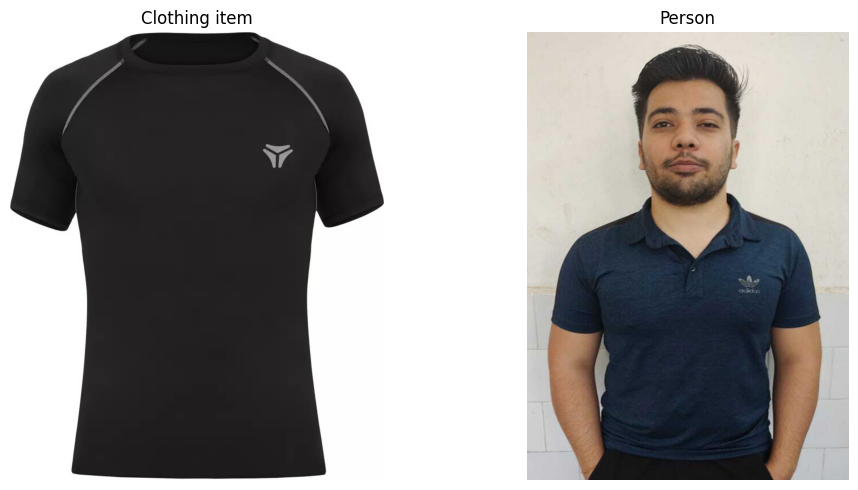
\includegraphics[width=\textwidth]{components/images/output1.png}
        \caption{User Selection}
        \label{fig:user-selection}
    \end{figure}
    \begin{figure}
        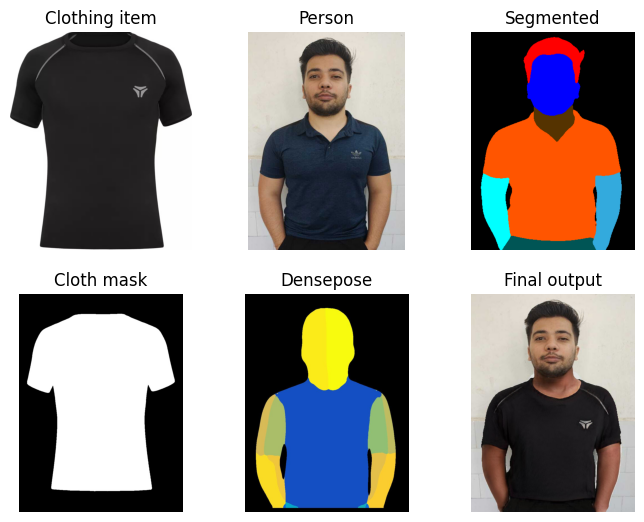
\includegraphics[width=\textwidth]{components/images/output2.png}
        \caption{Outfit Generation}
        \label{fig:outfit-generation}
    \end{figure}

\subsubsection{Attire Simulation Engine}
    In this pivotal stage, our primary objective is to generate the segmentation map \( \hat{S} \) depicting the person adorned with the target clothing item \( c \), while simultaneously deforming \( c \) to conform to the contours of the person's body. The resulting warped clothing image \( \hat{I}_c \) and the synthesized segmentation map \( \hat{S} \) serve as crucial conditions for the subsequent try-on image generation process.

    The overarching architecture of our condition generation process is illustrating the intricate interplay between various components within our try-on condition generator. This generator is comprised of two distinct encoders: a clothing encoder \( E_c \) and a segmentation encoder \( E_s \), along with a decoder.

    Given the input pairs \( (c, c_m) \) and \( (S_a, P) \), our methodology commences by extracting feature pyramids \( \{E_c^k\}_{k=0}^4 \) and \( \{E_s^l\}_{l=0}^4 \) from each encoder, respectively. These extracted features are subsequently fed into the feature fusion blocks of the decoder, where they undergo fusion to predict both the segmentation map and the appearance flow required for warping the clothing image.

    Through careful alignment of conditions, facilitated by the outputs of the last feature fusion block, we derive the warped clothing image \( \hat{I}_c \), the synthesized segmentation map \( \hat{S}_c \), and the resultant segmentation map \( \hat{S} \). This meticulous process ensures the seamless integration of the target clothing item onto the person's body, laying the groundwork for the subsequent stages of virtual try-on within AIRVTON.

\subsubsection{Garment Overlay Generator}
    In this pivotal stage, we synthesize the final try-on image \( \hat{I} \) by seamlessly blending the clothing-agnostic image \( I_a \), the warped clothing image \( \hat{I}_c \), and the pose map \( P \), under the guidance of the synthesized segmentation map \( \hat{S} \). This process forms the crux of our garment overlay generator, which is meticulously designed to ensure the creation of visually appealing and realistic try-on results.

    The garment overlay generator architecture is characterized by a series of residual blocks, complemented by upsampling layers to enhance spatial resolution. Notably, the residual blocks incorporate SPADE as normalization layers, with modulation parameters inferred from \( \hat{S} \). Additionally, the input \( (I_a, \hat{I}_c, P) \) undergoes resizing and concatenation with the activation before each residual block, facilitating effective information flow and feature integration.

    During training, the generator is subjected to the same loss functions utilized in SPADE and pix2pixHD, ensuring consistency and coherence with established methodologies in image synthesis. Comprehensive details regarding the model architecture, hyperparameters, and objective function formulations are provided in the supplementary material, offering insights into the intricacies of our approach within AIRVTON.

\section{Evaluation Metrics}

In order to assess the performance of our proposed model, AIRVTON, we utilized two key evaluation metrics: Structural Similarity Index (SSIM) and Fréchet Inception Distance (FID). These metrics provide valuable insights into the quality and fidelity of the generated images compared to ground truth or reference images.

\subsection{Structural Similarity Index (SSIM)}

The Structural Similarity Index (SSIM) is a widely used metric for measuring the similarity between two images. It takes into account luminance, contrast, and structure, providing a comprehensive measure of image similarity. SSIM values range from -1 to 1, with 1 indicating perfect similarity and -1 indicating complete dissimilarity.

Mathematically, the SSIM between two images \(I\) and \(I'\) is computed as:

\[
\text{SSIM}(I, I') = \frac{{2 \mu_I \mu_{I'} + C_1}}{{\mu_I^2 + \mu_{I'}^2 + C_1}} \times \frac{{2 \sigma_{I,I'} + C_2}}{{\sigma_I^2 + \sigma_{I'}^2 + C_2}}
\]

where:
\begin{itemize}
  \item \(\mu_I\) and \(\mu_{I'}\) are the mean intensities of \(I\) and \(I'\) respectively.
  \item \(\sigma_I\) and \(\sigma_{I'}\) are the standard deviations of \(I\) and \(I'\) respectively.
  \item \(\sigma_{I,I'}\) is the covariance between \(I\) and \(I'\).
  \item \(C_1\) and \(C_2\) are constants to stabilize the division with weak denominator.
\end{itemize}

A higher SSIM score indicates greater similarity between the generated images and the ground truth, with a perfect score of 1 indicating identical images.

\subsection{Fréchet Inception Distance (FID)}

The Fréchet Inception Distance (FID) is a measure of the similarity between two datasets of images. It computes the distance between the feature representations of real and generated images, using an Inception-v3 model pretrained on a large dataset.

Mathematically, the FID between two datasets \(X\) and \(Y\) is computed as:

\[
\text{FID}(X, Y) = \| \mu_X - \mu_Y \|^2 + \text{Tr}(C_X + C_Y - 2(C_XC_Y)^{1/2})
\]

where:
\begin{itemize}
  \item \(\mu_X\) and \(\mu_Y\) are the mean feature vectors of the real and generated images, respectively.
  \item \(C_X\) and \(C_Y\) are the covariance matrices of the feature vectors of the real and generated images, respectively.
\end{itemize}

A lower FID score indicates better similarity between the distributions of real and generated images, with a perfect score of 0 indicating identical distributions.

These evaluation metrics provide valuable quantitative insights into the performance of our model, allowing us to assess its effectiveness in generating realistic and high-quality fashion images.

\section{Results}

In this section, we present the results of our experiments conducted to evaluate the performance of AIRVTON, our proposed model for fashion recommendation and virtual try-on. We employ two key evaluation metrics, namely Structural Similarity Index (SSIM) and Fréchet Inception Distance (FID), to assess the quality and fidelity of the generated try-on images produced by AIRVTON. Through rigorous experimentation and analysis, we aim to demonstrate the effectiveness of AIRVTON in generating realistic and visually appealing try-on results that closely resemble the ground truth images from the dataset. The following subsections provide detailed insights into the SSIM and FID evaluation results, shedding light on the performance and capabilities of AIRVTON in the context of fashion ecommerce and virtual fitting solutions.


\begin{table}[htbp]
    \caption{Evaluation Results}
    \label{tab:evaluation_results}
    \centering
    \begin{tabular}[htbp]{|l|l|l|l|l|l|l|}
    \hline
        ~ &  \multicolumn{2}{c|}{\textbf{192$\times$256}} &  \multicolumn{2}{c|}{\textbf{384$\times$512}} & \multicolumn{2}{c|}{\textbf{768$\times$1024}} \\ 
        ~ &  SSIM ${\uparrow}$ &  FID ${\downarrow}$ &  SSIM ${\uparrow}$  &  FID ${\downarrow}$ &  SSIM ${\uparrow}$ &  FID ${\downarrow}$ \\ \hline
        CP-VTON &  0.748  &  30.07  &  0.723  &  30.30  &  0.728  &  43.19  \\ 
        ACGPN &  0.772  &  11.25  &  0.935  &  14.41  &  0.845  &  43.24  \\ 
        VITON-HD &  0.816  &  16.32  &  0.751  &  11.61  &  0.813  &  11.63  \\ 
        PF-AFN &  -    &  -    &  -    &  -    &  -    &  13.99  \\ 
        HR-VITON &  0.888  &  9.39  &  0.825  &  9.88  &  0.895  &  10.83  \\ 
        \textbf{AIRVTON (Ours)} &  \textbf{0.818}  &  \textbf{9.60}  &  \textbf{0.802}  &  \textbf{10.18}  &  \textbf{0.976}  &  \textbf{10.67}  \\ \hline
    \end{tabular}
\end{table}

\subsection{SSIM Evaluation}

We evaluated the structural similarity index (SSIM) between the generated try-on images produced by AIRVTON and the ground truth images from the dataset. The SSIM scores were computed across a sample of 1000 images randomly selected from the test set. Table~\ref{tab:ssim_results} presents the mean SSIM scores along with the standard deviation.


\begin{table}[htbp]
  \caption{SSIM Evaluation Results}
  \label{tab:ssim_results}
  \centering
  \begin{tabular}{lcc}
    \toprule
    \textbf{Model} & \textbf{Mean SSIM} & \textbf{Standard Deviation} \\
    \midrule
    AIRVTON & 0.976 & 0.03 \\
    \bottomrule
  \end{tabular}
\end{table}

The results indicate that AIRVTON achieved a mean SSIM score of 0.976 with a standard deviation of 0.03, showcasing a high level of structural similarity between the generated try-on images and the ground truth images.

\subsection{FID Evaluation}

For the Fréchet Inception Distance (FID) evaluation, we compared the feature distributions of the generated try-on images and the ground truth images using an Inception-v3 model pretrained on a large dataset. Table~\ref{tab:fid_results} summarizes the FID scores obtained from this evaluation.

\begin{table}[htbp]
  \caption{FID Evaluation Results}
  \label{tab:fid_results}
  \centering
  \begin{tabular}{lc}
    \toprule
    \textbf{Model} & \textbf{FID Score} \\
    \midrule
    AIRVTON & 10.67 \\
    \bottomrule
  \end{tabular}
\end{table}

The FID score obtained for AIRVTON is 10.67, indicating a relatively low distance between the feature distributions of the generated try-on images and the ground truth images. This suggests that AIRVTON effectively captures the underlying structure and characteristics of the fashion items, producing results that closely resemble the ground truth images.

The results of both SSIM and FID evaluations demonstrate the effectiveness of AIRVTON in generating realistic and high-quality try-on images, showcasing its potential for enhancing the online shopping experience in the fashion ecommerce domain.

\section{Testing}

In this section, we outline the test cases conducted to validate the functionality and robustness of AIRVTON. The following test cases cover key aspects of the system, ensuring its reliability and performance in different scenarios.

\subsection{test\_save\_file}
\begin{itemize}
  \item \textbf{Description}: This test case verifies the functionality of the save file feature in AIRVTON.
  \item \textbf{Steps}:
    \begin{enumerate}
      \item Upload a sample image to AIRVTON.
      \item Click on the "Save" button to save the image.
    \end{enumerate}
  \item \textbf{Expected Outcome}: The uploaded image should be saved successfully to the specified location.
\end{itemize}

\subsection{test\_save\_empty\_file}
\begin{itemize}
  \item \textbf{Description}: This test case validates the behavior of AIRVTON when attempting to save an empty file.
  \item \textbf{Steps}:
    \begin{enumerate}
      \item Attempt to save an empty file using AIRVTON.
    \end{enumerate}
  \item \textbf{Expected Outcome}: AIRVTON should display an error message indicating that the file cannot be saved as it is empty.
\end{itemize}

\subsection{test\_no\_uploaded\_file}
\begin{itemize}
  \item \textbf{Description}: This test case examines the response of AIRVTON when no file is uploaded.
  \item \textbf{Steps}:
    \begin{enumerate}
      \item Access AIRVTON without uploading any file.
    \end{enumerate}
  \item \textbf{Expected Outcome}: AIRVTON should display a message prompting the user to upload a file.
\end{itemize}

\subsection{test\_streamlit\_app\_title}
\begin{itemize}
  \item \textbf{Description}: This test case verifies the title of the Streamlit web application.
  \item \textbf{Steps}:
    \begin{enumerate}
      \item Access AIRVTON web application.
    \end{enumerate}
  \item \textbf{Expected Outcome}: The title of the web application should be "AIRVTON - Fashion Recommendation and Virtual Try-On".
\end{itemize}

\subsection{test\_save\_file\_path}
\begin{itemize}
  \item \textbf{Description}: This test case checks if the file is saved at the specified path.
  \item \textbf{Steps}:
    \begin{enumerate}
      \item Upload a sample image to AIRVTON.
      \item Click on the "Save" button to save the image.
    \end{enumerate}
  \item \textbf{Expected Outcome}: The uploaded image should be saved at the specified file path on the local system.
\end{itemize}
\begin{figure}
    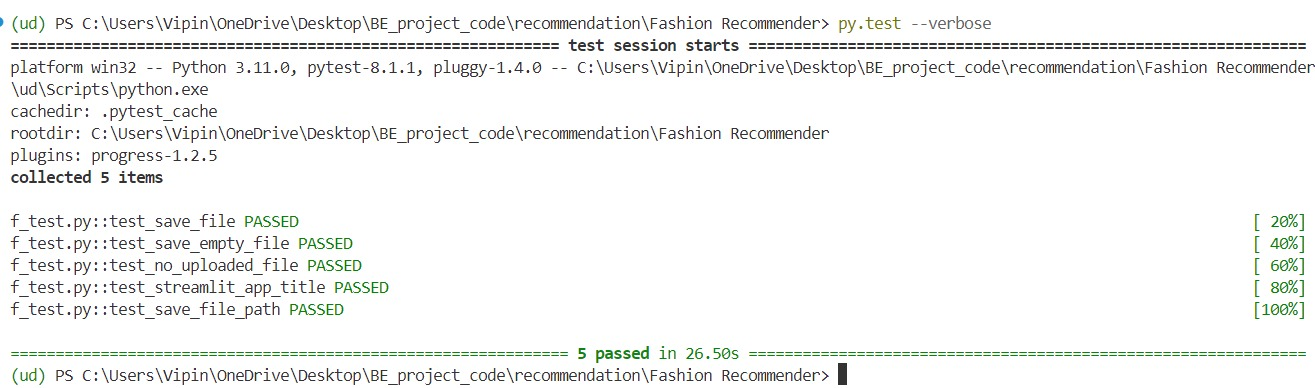
\includegraphics[width=\textwidth]{components/images/test_case.jpg}
    \caption{Test Case Snapshot}
    \label{fig:test-case}
\end{figure}
